\documentclass[a4paper,12pt]{article}
\usepackage[OT4,plmath]{polski}
\usepackage[utf8x]{inputenc}
\usepackage{url}

\usepackage{a4wide}
\usepackage{hyperref}
\usepackage{caption}
\usepackage{graphicx}

\graphicspath{ {imgs/} }

\title{{\textbf{Skalowanie baz danych na przykładzie MySQL}}}
\author{Rafał Łasocha}
\date{Wrocław, \today\ r.}

% Wdowy, sieroty
% \clubpenalty=9996
% \widowpenalty=9999
% \brokenpenalty=4991
% \hyphenpenalty=5000
% \predisplaypenalty=10000
% \postdisplaypenalty=1549
% \displaywidowpenalty=1602

\begin{document}

\maketitle

\section{Skalowanie systemów informatycznych}

Dla wielu aplikacji wystarczy pojedynczy serwer bazodanowy. Niektóre z nich zbierają jednak tyle informacji, że prędzej czy później dochodzi do sytuacji, w której jeden serwer nie jest w stanie obsłużyć wszystkich żądań w akceptowalnym czasie. Rozwiązaniem tego problemu jest skalowanie systemu bazodanowego.

\subsection{Co to znaczy, że system jest skalowalny?}

Twórcy usług bazodanowych (lub innych usług, z których korzystają aplikacje), często posługują się terminem „skalowalność” w odniesieniu do swoich produktów. Mimo to, że~ten~termin ma znaczenie marketingowe, można go w miarę konkretnie zdefiniować. 

Najpierw zdefiniujmy pojęcie „wydajności” systemu. Dokładna definicja wydajności systemu baz danych w znacznym stopniu zależy od sposobu jego wykorzystania. Różne aplikacje mają różny stosunek zapisów do odczytów, różne wielkości tabel (w~niektórych systemach wszystkie tabele są mniej więcej jednakowo duże, w innych jest tylko kilka tabel, które składają się na większość systemu i to czas odpowiedzi odczytów lub zapisów tych kilku tabel próbujemy zoptymalizować) itd. Intuicyjnie możemy myśleć~o wydajności w~ten~sposób: jak dużą możemy osiągnąć przepustowość (na przykład w liczbie zapytań na~sekundę) utrzymując rozsądny czas odpowiedzi.

Dla przykładu, popularne testy wydajnościowe typu „wyślemy milion zapytań SQL i~policzymy czas, w którym serwer obsłuży wszystkie zapytania” to nie jest do końca to, co nas interesuje, bo w takim przypadku serwer będzie przetwarzał zapytania pod maksymalnym obciążeniem. Nas interesuje test „będziemy wysyłać tysiąc zapytań na minutę i~dostaniemy odpowiedź poniżej 3 ms w 90\% przypadków”. Należy podkreślić, że wydajność bardzo zależy od konkretnego systemu, ponieważ wspomniane „tysiąc zapytań na minutę” nie są dowolnymi zapytaniami, tylko takimi, które występują w testowanej aplikacji. Stąd, na wydajność testowanej aplikacji ma wpływ liczba użytkowników, wielkość przechowywanych danych na serwerze, wielkość przechowywanych danych w przeliczeniu na jednego użytkownika („prawo papieża”: zawsze może korzystać z aplikacji kilku użytkowników, na~których przypada nieproporcjonalnie dużo danych --- i to też musimy wziąć pod uwagę, bo papież również chciałby korzystać swobodnie z aplikacji).

Poczas rozwoju aplikacji często okazuje się, że aktualna wydajność systemu bazodanowego jest niewystarczająca. Tutaj możemy przejść do definicji skalowalności. Skalowalność mówi nam, do jakiego stopnia zwiększa się wydajność systemu, gdy dodajemy kolejne serwery. Może się wydawać, że gdy mamy jeden serwer i dodamy drugi, to wydajność zwiększy się o 100\% (skalowalność liniowa --- Rysunek  \ref{fig:scaling-linear}). Jednak najczęściej dodanie drugiego serwera nie da nam idealnego zrównoleglenia, bo prawdopodobnie jest jakaś część pracy, której nie da się zrównoleglić. Dlatego skalowalność wielu systemów można zobrazować krzywą trochę poniżej liniowej, a prawo uwzględniające fakt, że części pracy nie możemy zrównoleglić, nazywamy prawem skalowalności Amdahla.

\begin{figure}[ht]
\centering
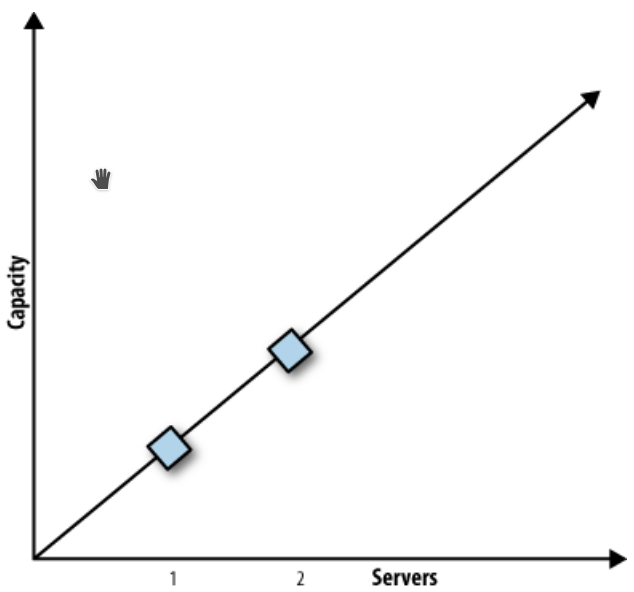
\includegraphics[width=0.5\textwidth]{scaling-linear.png}
\caption{Skalowalność liniowa}
\label{fig:scaling-linear}
\end{figure}

\begin{figure}[ht]
\centering
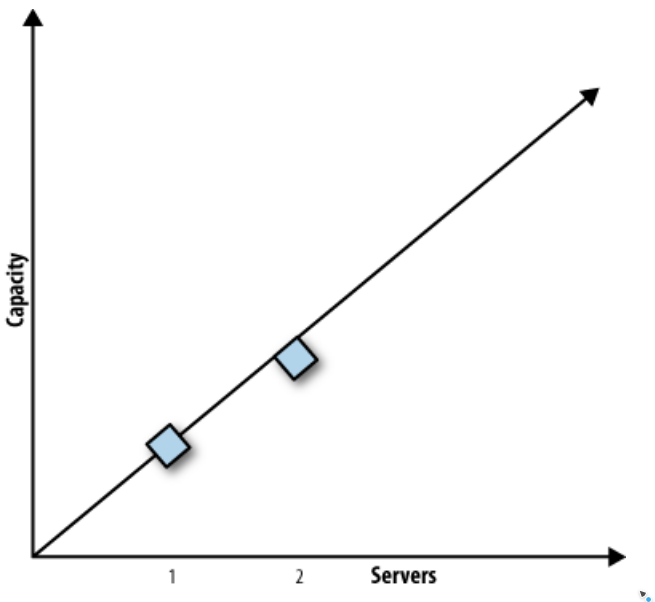
\includegraphics[width=0.5\textwidth]{scaling-almost-linear.png}
\caption{Skalowalność Amdahla}
\label{fig:scaling-almost-linear}
\end{figure}

Intuicja może nam podpowiadać, że systemy mają prawdopodobnie jakieś granice, do~którego możemy dodawać dodatkowe serwery i  tym sposobem zwiększać wydajność. Dlatego też Neil J. Gunther sformułował uniwersalne prawo skalowalności, które bierze również pod uwagę fakt, że serwery w klastrze muszą wymieniać ze sobą informacje (na~zasadzie „każdy z każdym”). Ta komunikacja pomiędzy serwerami powoduje, że do wykonania jest $N^2$ dodatkowej pracy (gdzie $N$ to liczba serwerów), więc istnieje taka liczba serwerów w klastrze, gdy dodanie kolejnego serwera pogorszy wydajność całego systemu (Rysunek~\ref{fig:scaling-all})!

\begin{figure}[ht]
\centering
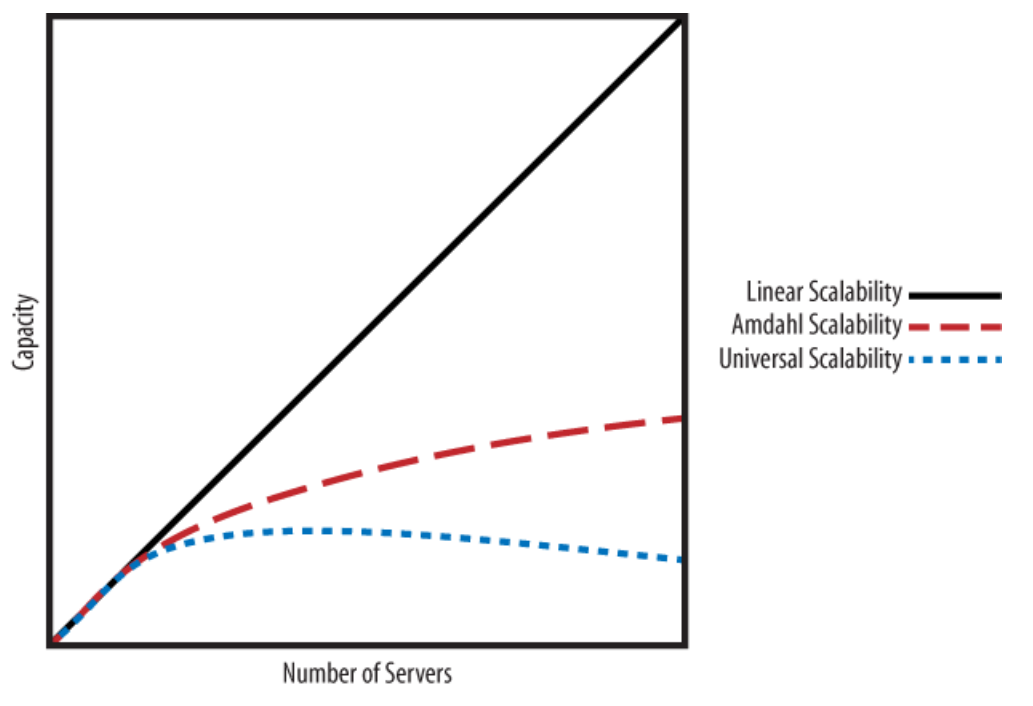
\includegraphics[width=0.7\textwidth]{scaling-all.png}
\caption{Wszystkie popularne rodzaje skalowalności}
\label{fig:scaling-all}
\end{figure}


Większość systemów przestrzega właśnie uniwersalnego prawa skalowalności. Oczywiście jak każdy model, jest to tylko przybliżenie --- niektóre systemy mogą nie potrzebować akurat $N^2$ dodatkowej pracy na komunikację, tylko inną funkcję. Może się zdarzyć też, że~skalowalność będzie większa niż liniowa (rozpatrzmy przypadek, gdy mamy jeden serwer z szamotającymi się procesami, który ma obciążoną zarówno pamięć jak i dysk twardy, po czym dodajemy drugi serwer, dzięki któremu wszystkie dane mieszczą się w pamięci).

\subsection{Skalowanie MySQL}

Rozważymy dwa sposoby na skalowanie systemu bazodanowego --- skalowanie pionowe i~skalowanie poziome. Skalowanie pionowe polega na tym, że ciągle mamy tylko jeden serwer, ale zwiększamy jego parametry (pamięć RAM, liczba CPU), żeby był bardziej wydajny. W~skalowaniu poziomym, zwiększamy liczbę maszyn.

\section{Skalowanie pionowe}

Skalowanie pionowe jest świetnym rozwiązaniem, aby „kupić” sobie trochę czasu. Jeśli~jeszcze nie wiemy, czy nasza aplikacja odniesie sukces, skalowanie pionowe jest lepszym wyborem, bo kosztuje znacznie mniej --- zmiana maszyny na lepszą wymaga mniejszych udziałów pracy personelu IT niż skonfigurowanie całej infrastruktury, przygotowanie aplikacji do korzystania z wielu serwerów, przygotowanie procedur tworzenia/przywracania kopii zapasowych itd. A ponieważ z reguły największym składnikiem kosztów działalności firmy są wynagrodzenia personelu IT, to skalowanie pionowe jest bardziej opłacalne.

Główną wadą skalowania pionowego jest fakt, że nie można go stosować w nieskończoność. Parametry serwerów mają swoje rozsądne granice i im lepsze serwery kupujemy, tym~droższe stają się zasoby, więc w pewnym momencie zaczyna się opłacać przejście na skalowanie poziome. Ponadto, zaleta skalowania pionowego polegająca na oszczędzeniu kosztów konfiguracji nie zawsze działa --- czasami tylko wymiana sprzętu nie prowadzi do dużego zwiększenia wydajności i tak czy inaczej potrzebujemy poświęcić trochę czasu personelu IT na skonfigurowanie bazy danych do nowego sprzętu.

\section{Skalowanie poziome}

Skalowanie poziome możemy podzielić na trzy rodzaje: replikację, dzielenie funkcjonalne i~\textit{sharding} (podzielenie jednej bazy na kilka mniejszych wg określonego klucza). Replikacja jest najprostszą formą i pozwala przenieść część odczytów na inne serwery, ale nie pomoże nam, jeśli naszym wąskim gardłem są zapisy. Zarówno dzielenie funkcjonalne jak i \textit{sharding} rozwiązuje problem wydajności zapisów.

\section{Dzielenie funkcjonalne}

Dzielenie funkcjonalne jest prostym pomysłem, niezależnym od konkretnej bazy danych~i~jej możliwości (w przeciwieństwie do np. replikacji, która musi być wspierana przez bazę danych, żeby ją efektywnie wdrożyć). Jeśli nasza aplikacja jest niewydajna, to być może aplikacja obsługuje zbyt wiele funkcjonalności. Możemy ją więc podzielić na dwie aplikacje, ze~względu na rozdzielne zestawy funkcjonalności, jeśli kod tych dwóch aplikacji korzysta w dużej mierze z rozdzielnych zestawów tabel.

Rozważmy dla przykładu serwis informacyjny. Możemy bazę danych podzielić na kilka oddzielnych dużych funkcjonalności: witryna z bieżącymi wiadomościami, forum dla~czytelników, wsparcie dla użytkownika i właśnie baza użytkowników. Udało nam się więc niewielkim kosztem podzielić serwis na kilka baz danych i prawdopodobnie osiągnąć skalowalność bliską liniowej (bazy danych są całkowicie rozłączne i nie komunikują się ze sobą). Jak widać dzielenie funkcjonalne jest względnie proste (w porównaniu do \textit{shardingu}, który będzie opisany w dalszej części artykułu) i nie niesie ze sobą zbyt wielu zagrożeń (w chwili gdy rzeczywiście musimy porozmawiać z więcej niż jedną bazą danych, być może musimy się pogodzić z brakiem transakcyjności --- ale jeśli dzielenie funkcjonalne jest zrobione poprawnie, to są to rzadkie przypadki).

Niestety prędzej czy później zabraknie w naszej aplikacji modułów, które jest łatwo wyciągnąć do osobnych aplikacji, korzystających z osobnych baz danych. W szczególności, może się okazać, że tylko niektóre z tych już rozdzielonych baz danych potrzebują bardziej skomplikowanego rozwiązania (\textit{shardingu}), więc z reguły dzielenie funkcjonalne idzie w~parze z \textit{shardingiem} i \textit{sharding} tego podziału nie zastępuje.

\section{Sharding}

Jest to obecnie najpopularniejsza metoda skalowania bazy danych MySQL. Wystarczy wspomnieć, że korzystają z tego rozwiązania takie firmy jak Facebook, Instagram czy Uber. Jak wspomniano wyżej, \textit{sharding} idzie w parze z dzieleniem funkcjonalnym. Z reguły jest jakaś baza danych, która przechowuje dane globalne potrzebne wszystkim (np.~właśnie listę użytkowników), często za klastrem szybkiego cache (np. memcached). Aplikacje które korzystają z bazy danych z \textit{shardingiem}, są pisane z uwzględnieniem tego faktu. Jest potrzebna jakaś programistyczna abstrakcja, która decyduje, do jakiego serwera bazodanowego wysłać żądania SQL. Można to zrobić tak, aby kod nie zależał od tego czy baza danych korzysta z \textit{shardingu} czy nie (przez bibliotekę z wysokopoziomowym API nieujawniającą tego faktu), ale jest to niewskazane. Powoduje to nieprzemyślaną, równomierną (ilościowo) dystrybucję danych po wszystkich serwerach, która jest nieefektywna (co pokażemy później), więc chcemy robić to trochę mądrzej.

\subsection{Wybór klucza shardującego}

Jeśli uznamy że potrzebujemy \textit{shardingu}, jedną z pierwszych decyzji do podjęcia jest wybór klucza shardującego. Klucz ten decyduje, w jakim shardzie zostanie umieszczony rekord. W~MySQL NDB Cluster, który jest gotowym rozwiązaniem do wdrażania shardowanej bazy danych, rekordy są równomiernie rozprowadzane pomiędzy serwerami według haszowanego klucza głównego w danej tabeli. To jest proste, ale niezbyt wydajne rozwiązanie.

Rozważmy teraz platformę blogową, której użytkownicy publikują wpisy i komentują wpisy innych autorów. Żeby wyświetlić stronę główną takiego bloga, musimy pobrać wszystkie wpisy danego użytkownika. Skoro wpisy są rozłożone równomiernie na wszystkich serwerach, to musimy zrobić (najlepiej równolegle) zapytania do wszystkich serwerów i potem połączyć te dane (dodatkowe utrudnienia: co, jeśli zapytanie miało klauzulę \texttt{ORDER~BY}, \texttt{LIMIT}, \texttt{HAVING} --- to wszystko musi być wtedy obsłużone w abstrakcji programistycznej po stronie klienta). Jest to oczywiście możliwe do zrobienia, ale być może chcielibyśmy odpytać jak najmniej maszyn (choćby dlatego, że wszystkie zapytania są~podatne na błędy sieciowe). Dlatego najczęściej dobrym kluczem jest identyfikator użytkownika (jeśli myślimy np.~o~witrynie społecznościowej) lub identyfikator klienta (częste w aplikacjach modelu~SaaS).

Mamy tutaj jeszcze inny problem. Załóżmy że mamy dwa widoki:
\begin{itemize}
 \setlength{\itemsep}{0.06cm}
 \setlength{\parskip}{0.06cm}
 \item wyświetlenie wpisu i wszystkie komentarze do niego od innych użytkowników,
 \item wyświetlenie profilu użytkownika, ze wszystkimi jego komentarzami.
\end{itemize}
Na którym serwerze przechowywać w takim przypadku komentarze? Możemy to zrobić według identyfikatora użytkownika lub identyfikatora wpisu, ale wtedy zawsze jeden z powyższych widoków będzie wymagał zapytań do wszystkich serwerów. Częstym rozwiązaniem jest tutaj denormalizacja i duplikacja danych. Oczywiście, przechowywanie zduplikowanych danych wiąże się z pewnym kosztem, ale w naszym przypadku wydajność jest być może ważniejsza. Można też się zastanowić, czy na pewno wszystkie dane o komentarzach są~potrzebne w obu zastosowaniach. Może w przypadku profilu użytkownika wystarczy wyświetlić jedynie nagłówki komentarzy? Wówczas przechowujemy dane dokładnie zgodne z ich przeznaczeniem, co jest dodatkową zaletą tego rozwiązania.

\subsection{Zapytania do wielu shardów}

Niezależnie od zastosowanych technik, nigdy nie uda się nam wybrać klucza, który by idealnie podzielił dane tak, że wszystkie zapytania odwoływałyby się tylko do jednego sharda. Jeśli na naszej platformie blogowej chcielibyśmy wyświetlić listę najpopularniejszych postów, siłą rzeczy musielibyśmy wysłać zapytania do wszystkich shardów. Jest kilka technik radzenia sobie z takimi zapytaniami:
\begin{itemize}
 \setlength{\itemsep}{0.06cm}
 \setlength{\parskip}{0.06cm}
 \item warstwa cache dla kosztownych zapytań,
 \item tabele, które przechowują wyniki trudniejszych zapytań. Dane o najpopularniejszych postach możemy na bieżąco przetwarzać w tle i dodać je do tabeli z wynikami. Taką tabelę z wynikami możemy wtedy albo zduplikować na wszystkich shardach, albo wstawić do oddzielnej bazy danych.
\end{itemize}

Nie tylko zapytania są trudne do zrealizowania w shardowanych bazach danych. Jeśli stosujemy \textit{sharding}, to tracimy też klucze obce (pomiędzy shardami) i transakcyjność (zależnie od rozwiązania są jednak sposoby, aby transakcyjność odzyskać).

Poza odczytem danych trudniejsze też może być ich usunięcie. W dużej aplikacji jeden użytkownik jest powiązany z wieloma rekordami w różnych tabelach, więc usunięcie ich może trwać dłużej, niż byśmy akceptowali. Dlatego jeśli chcemy usunąć użytkownika, to~zamiast wysyłać żądania usunięcia danych do wszystkich shardów natychmiast, możemy tylko zakolejkować użytkownika do usunięcia w jakimś zewnętrznym procesie, a samym usuwaniem danych zajmie się ten proces działający w tle.

\subsection{Przydzielanie shardów do serwerów}

Niekoniecznie musi być tak, że na jednym serwerze jest tylko jeden shard z danymi. Przeciwnie, lepszym pomysłem jest posiadanie wielu małych shardów na każdym serwerze. Poniżej przedstawię zalety i wady obu rozwiązań.

Wyobraźmy sobie, że mamy na serwerze 100GB danych. Możemy je podzielić na 1 shard 100 GBajtowy lub 100 shardów wielkości 1GB. Pierwszą sprawą, którą można wziąć pod uwagę, to zmiany struktury tabel. W MySQL wiele z operacji zmian struktury, takie jak np. zmiana długości pola VARCHAR, dodawanie niektórych indeksów, dodawanie kolumn w wersji niższej niż 5.6 itd blokuje całą tabelę. Lepiej więc, aby proces zmiany struktury był wykonywany po kolei i blokował każdy mały shard na kilka minut, niż żeby jeden duży shard został zablokowany na godzinę. Mniejsze shardy są też łatwe do przenoszenia, bo operacja przeniesienia jednego shardu na drugi jest znacznie prostsza niż operacja rozdzielenia sharda na kilka części.

Są tylko dwie wady małych shardów: po pierwsze rośnie zwykle liczba zapytań pomiędzy różnymi shardami (z którą nauczyliśmy się sobie radzić w poprzedniej sekcji). Drugą wadą jest to, że jeśli mamy aktualnie działającą aplikację i dochodowy biznes, operacja rozdzielenia bazy na dwie części (i dodanie odpowiedniej infrastruktury) może być znacznie prostsza niż rozdzielenie bazy na 1000 części. W pierwszym przypadku pewnie możemy sobie jeszcze pozwolić na wykonywanie pewnych operacji dwukrotnie, w drugim koniecznie musimy zautomatyzować wszystkie operacje działające na bazie danych.

\subsection{Implementacja shardów na serwerach}

Jak reprezentować shard danych na serwerze? Jest kilka najpopularniejszych sposobów:

\begin{itemize}
 \setlength{\itemsep}{0.06cm}
 \setlength{\parskip}{0.06cm}
 \item każdy shard jest osobną bazą danych o takiej samej nazwie jak oryginalna,
 \item każdy shard jest osobną bazą danych o nazwie z sufiksem numerycznym oznaczającym numer sharda (np. do tabeli z komentarzami w bazie danych \texttt{bookclub} odwoływalibyśmy się przez \texttt{bookclub\_23.comments} itd.),
 \item na jednym serwerze jest tylko jedna baza danych, a tabele mają sufiks numeryczny oznaczający numer sharda (np. \texttt{bookclub.comments\_23}),
 \item sufiks numeryczny oznaczający numer sharda jest zarówno w nazwie bazy danych, jak i nazwie tabeli (\texttt{bookclub\_23.comments\_23}),
 \item połączenie dowolnego z powyższych. Można też wziąć pod uwagę uruchomienie na~jednym serwerze kilku instancji MySQL.
\end{itemize}

Wszystkie podane sposoby są łatwe do wprowadzenia w nowej aplikacji, więc w nowych aplikacjach doradzane jest użycie sufiksu zarówno w tabeli, jak i bazie danych, żeby uniknąć ewentualnych pomyłek i błędów. Jednak jest to też sposób najbardziej inwazyjny dla kodu produkcyjnego. Dodanie numeru sharda tylko do bazy danych jest średnio inwazyjne w kodzie aplikacji, bo pewnie musimy ten numer gdzieś przekazać przy rozpoczęciu połączenia do serwera, ale kod wykonujący zapytania SQL może zostać taki, jaki był przed dodaniem \textit{shardingu} do aplikacji. Jeśli sufiks jest też w nazwie tabel, to zmian może być znacznie więcej --- prawdopodobnie każde zapytanie SQL w systemie będzie musiało być nieco zmodyfikowane.

Implementując algorytm dystrybucji shardów na serwerach, warto wziąć pod uwagę lokalizację użytkownika. Jeśli nasza firma jest globalna, użytkowników z Europy można umieścić w innej serwerowni (zlokalizowanej w Europie), niż użytkowników z Azji.

\subsection{Metody przydzielania rekordów do shardów}

Musimy jakoś rozdzielić wszystkie rekordy w bazie danych na różne shardy. Szukamy więc funkcji, która po zaaplikowaniu do klucza shardującego zwraca numer sharda na którym mamy umieścić dany rekord.

\subsection{Przydział statyczny}

Pierwsze co przychodzi na myśl, to jakaś funkcja haszująca i operacja modulo. Przykładowo, jeśli klucz sharda to 111 i mamy 100 shardów, to możemy (pomijając funkcję haszującą) przydzielić temu kluczowi shard 11 ($111 \bmod 100 = 11$). Zaletami tego rozwiązania jest prostota i wydajność. Przydział statyczny ma istotne wady:

\begin{itemize}
 \setlength{\itemsep}{0.06cm}
 \setlength{\parskip}{0.06cm}
 \item jeśli mamy tylko kilka shardów, to ciężko je zbalansować (może się okazać, że większość aktywnych użytkowników zostanie umieszczona na jednym shardzie),
 \item ciężko zmieniać liczbę shardów. Wymagałoby to operacji przenosin wszystkich rekordów do shardów z nowym identyfikatorem, co nie jest infrastrukturalnie prostą sprawą.
\end{itemize}

Z tych powodów, wiele firm, które najpierw wdrażają przydział statyczny (bo jest prosty do zrobienia) prędzej czy później przechodzi na przydział dynamiczny.

\subsection{Przydział dynamiczny}

Przydział dynamiczny polega na przechowywaniu całego odwzorowania z identyfikatora shardowania do numeru shardu w oddzielnym kontenerze z danymi (np. warstwa memcached, redisa, albo po prostu oddzielna baza danych). Wystarczy pamiętać, aby przy dodawaniu nowego użytkownika dodać też rekord do tego odwzorowania. Jak widać dodawanie nowych shardów jest całkowicie trywialne (nie wymaga właściwie żadnej ingerencji w~odwzorowanie), a przenoszenie użytkowników jest znacznie ułatwione. Korzystając z~przydziału dynamicznego możemy też sobie pozwolić na posiadanie shardów o różnej wielkości (jeśli akurat jesteśmy w trakcie aktualizacji serwerów do takich o większej mocy). Możemy też optymalizować dane rozmieszczając je dowolnie pomiędzy shardy, dzięki czemu jesteśmy w stanie zastąpić zapytania które wcześniej musiały być wysłane do wszystkich shardów takim, które musi zostać wysłane tylko do kilku (lub jednego).

\subsection{Przydział sprecyzowany}

Trzecim podejściem, trochę innym niż dwa poprzednie, jest przydział sprecyzowany. Zamiast odwzorowania przekształcającego klucz shardujący w numer sharda, możemy sprawić, żeby numer sharda zawierał się w kluczu shardującym (co trochę przypomina przydział statyczny). W tym celu, zakładając że kluczem shardującym jest identyfikator użytkownika, możemy np. założyć, że pierwsze 6 bitów identyfikatora użytkownika to właśnie numer sharda. Otrzymanie numeru sharda lub tej „rzeczywistej” części numeru użytkownika jest wtedy kwestią prostych operacji bitowych. Istotną zaletą tego rozwiązania jest fakt, że~nie~potrzebujemy żadnego dodatkowego zapytania aby otrzymać numer sharda. Jest~to~jakieś rozwiązanie pośrednie pomiędzy przydziałem stałym i dynamicznym, bo~możemy częściowo decydować, gdzie są nasze rekordy (podejmujemy decyzję o tym przy dodawaniu rekordu). Łatwo jest też zwiększyć liczbę używanych shardów. Wadą jest, podobnie jak w przydziale statycznym, trudność w przesuwaniu danych pomiędzy shardami. Jeśli dany rekord zostanie umieszczony w jakimś shardzie, to ciężko go będzie przenieść do~innego~shardu.

\section{Podsumowanie}

Omówiliśmy w tym artykule kilka technik skalowania bazy danych na przykładzie MySQL, zalety i wady skalowania pionowego i poziomego oraz zalety i wady różnego rodzaju decyzji, które trzeba podjąć przy skalowaniu poziomym.

Moje własne doświadczenie zawodowe jest jeszcze zbyt małe, bym mógł odnieść się do~całego tematu skalowania z praktycznego punktu widzenia. Największej aplikacji, przy której obecnie pracuję, wystarczy 16GB pamięci RAM i około 50GB dysku twardego. Minie jeszcze sporo czasu, zanim skalowanie pionowe i dzielenie funkcjonalne będzie niewystarczające i będziemy zmuszeni zaimplementować \textit{sharding}.

\section{Źródło}

Seminarium i referat oparłem na własnych doświadczeniach z programowaniem aplikacji korzystających z baz danych oraz na treści rozdziału 11 książki: Baron Schwartz, Peter Zaitsev, Vadim Tkachenko, „High Performance MySQL”, 3rd Edition, O'Reilly 2012.

\end{document}
